\documentclass[10pt]{beamer}
\hypersetup{pdfpagemode=FullScreen}
\usepackage[10pt]{moresize}
\usepackage{appendixnumberbeamer}
\usepackage{tcolorbox}
\usepackage{graphicx,wrapfig,lipsum}
\usepackage{booktabs}
\usepackage[scale=2]{ccicons}
\usepackage[utf8]{inputenc}
\usepackage{graphicx}
\usepackage{mdframed}
\usepackage{amsthm}
\usepackage{amsmath}
\usepackage{amscd}
\usepackage{fancyhdr}
\usepackage{listings}
\usepackage{framed}
\usepackage{xcolor}
\usepackage{amsmath}
\usepackage{pgfplots}
\usepackage[linguistics]{forest}
\usetheme{Frankfurt}
\usecolortheme{whale}
\usepgfplotslibrary{dateplot}
\usepackage{xspace}
\usepackage{hyperref}
\usepackage{mathrsfs}
\usepackage{svg}

\usepackage[
  separate-uncertainty = true,
  multi-part-units = brackets
]{siunitx}


\def\G{{\cal G}}

\def\mmu{\mbox{\boldmath $\mu$}}
\def\th{\mbox{\boldmath $\theta$}}
\def\Sig{\mbox{\boldmath $\Sigma$}}
\def\N{\mbox{\boldmath $N$}}





\def\0{\mbox{\boldmath $0$}}
\def\x{\mbox{\boldmath $x$}}
\def\u{\mbox{\boldmath $u$}}
\def\b{\mbox{\boldmath $b$}}
\def\y{\mbox{\boldmath $y$}}
\def\j{\mbox{\boldmath $j$}}
\def\s{\mbox{\boldmath $s$}}
\def\c{\mbox{\boldmath $c$}}
\def\a{\mbox{\boldmath $a$}}
\def\f{\mbox{\boldmath $f$}}
\def\g{\mbox{\boldmath $g$}}
\def\m{\mbox{\boldmath $m$}}
\def\1{\mbox{\boldmath $1$}}



\def\A{\mbox{\boldmath $A$}}
\def\X{\mbox{\boldmath $X$}}
\def\J{\mbox{\boldmath $J$}}
\def\L{\mbox{\boldmath $F$}}
\def\W{\mbox{\boldmath $W$}}
\def\B{\mbox{\boldmath $B$}}
\def\C{\mbox{\boldmath $C$}}
\def\V{\mbox{\boldmath $V$}}
\def\I{\mbox{\boldmath $I$}}
\def\J{\mbox{\boldmath $J$}}
\def\U{\mbox{\boldmath $U$}}

\def\calL{{\mathcal L}}
\def\calQ{{\mathcal Q}}
\def\calB{{\mathcal B}}


\def\tS{\tilde{\S}}
\def\tmu{\tilde{\mu}}
\def\td{\tilde{\d}}

\def\P{\mathbb{P}}
\def\E{\mathbb{E}}
\def\dd{\mathrm{d}}

\newcommand{\themename}{\textbf{\textsc{metropolis}}\xspace}
\newcommand\tab[1][1cm]{\hspace*{#1}}
\newcommand\tabsmall[1][0.2cm]{\hspace*{#1}}

\title[Master Thesis]{Automated classification of syllable types in vocal sequences of pups of the greater sac-winged bat Saccopteryx bilineata}
\author{Simon Hiller}

\institute{Andreas Fischer \&
Daniel Wegmann

University of Bern - Fribourg}
\date{28. February 2021}

\begin{document}

\begin{frame}
  \titlepage
\end{frame}

% Uncomment these lines for an automatically generated outline.
%\begin{frame}{Outline}
%  \tableofcontents
%\end{frame}

\section{Overview}

\begin{frame}{Intro}
\textbf{Around five years ago I initially become contact with the time-consuming workout of manual labeling the syllables in audio recording of vocalisation sequences.}
\end{frame}

\begin{frame}{How}
\begin{itemize}
\item Model: deep learning model with pattern searching abilities.
\item Approach: supervised learning
\begin{itemize}
\item Input: spectrogram
\item Output: corresponding syllable type
\end{itemize}
\end{itemize}
\end{frame}

\begin{frame}{Presentation Overview}
%\centering
\begin{itemize}
\item Introduction
\item Difficulties
\item Methods
\item Results
\item Discussion
\item Outlook
\item Questions
\end{itemize}
\end{frame}

\section{Introduction}
\begin{frame}{Language}
\begin{itemize}
\item How we become capable of learning language
\item Can language only be applied to human vocalisation
\end{itemize}
\end{frame}

\section{Difficulties}
\begin{frame}{Bioacoustic}
\begin{itemize}
\item Huge amount of recordings which needs to be labeled
\item How to normalize the recordings in respect to the place of recording
\item How to handle noise
\end{itemize}
\end{frame}

\begin{frame}{Syllables}
\begin{itemize}
\item Vary in size
\item Gradual change of a syllable type during development of pups vocalization
\item How to segment
\end{itemize}
\end{frame}

\section{Methods}
\begin{frame}{Overview}
\begin{figure}
\centering
    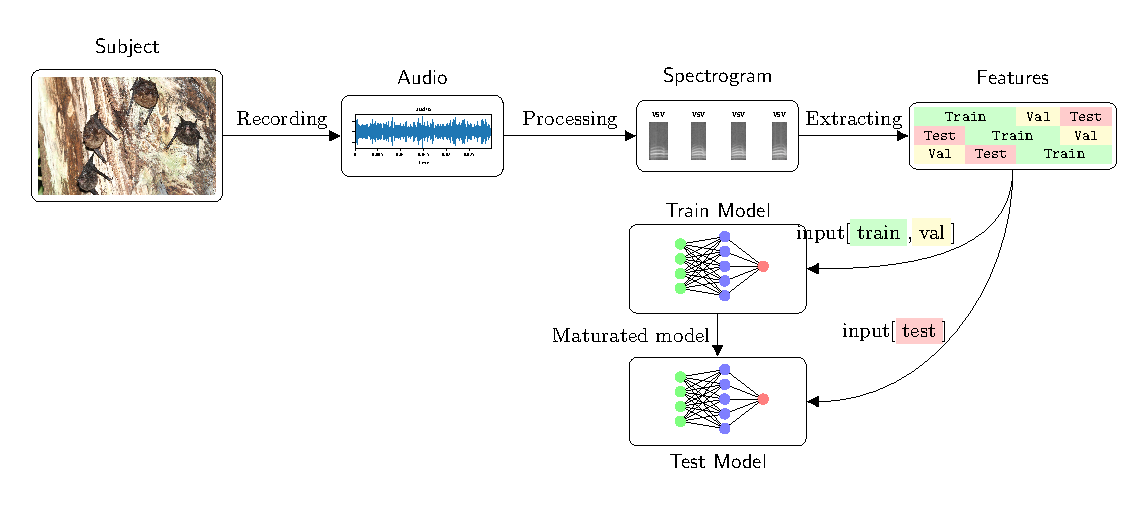
\includegraphics[width=1\linewidth]{image/pipeline.pdf}
    \caption{Flow diagram of the data.}
    \label{fig:pipeline}
\end{figure}
\end{frame}

\begin{frame}{Preprocessing overview}
\begin{itemize}
\item Filter out too short syllables and syllable types with not enough samples
\item Generate silent audio files per recording and create noise profiles with them
\item Extract audio parts which belongs to a syllable by the defined start and end time point
\item Left pad the extracted syllables to the same maximum length over all with the signal data from the background audio file
\item Apply noise reduction filter to the audio files based on the generated noise profiles.
\end{itemize}
\end{frame}

\begin{frame}{Preprocessing silent segmentation}
\begin{equation}\label{eq:silent_detection_1}
silent = \begin{cases} 1 & mse < mean(mse \text{ without label})+1, \\ 0 & \text{otherwise}. \end{cases}
\end{equation}
\begin{figure}
\centering
    \includesvg[inkscapelatex=false,width=1\textwidth]{image/silent_detection_sample1.svg}
    \caption{Plot of the result of the silence detection algorithm. The blackcurrant rectangles are the silent parts, on both sides the piece of \SI{5}{\milli\second} by which the silent parts were reduced is shown in transparent light blue. The yellow rectangle is a labelling part.}
    \label{fig:silent_detection_sample1}
\end{figure}
\end{frame}

\begin{frame}{Multilayer perceptron}
\begin{figure}[H]
\centering
  \includegraphics[width=1\textwidth]{image/mlp_schema.pdf}
  \caption{A diagram of a single perceptron, along with its position within a multilayer perceptron with fully connected layers.}
  \label{fig:mlp_schema}
\end{figure}
\end{frame}

\begin{frame}{Long short term memory}
\begin{figure}[H]
\centering
  \includegraphics[width=.7\textwidth]{image/lstm_schema.pdf}
  \caption{A diagram of a single LSTM cell and which values are recurrently used when processing a feature vector $x_1,\hdots,x_n$.}
  \label{fig:lstm_schema}
\end{figure}
\end{frame}


\begin{frame}{LSTM model}
\begin{figure}[H]
\centering
  \includegraphics[width=1\textwidth]{image/ml_model_lstm.pdf}\hfill
  \caption{Visualisation of the LSTM architecture. The size of the elements does not correspond exactly to their real dimension numbers.}
  \label{fig:ml_model_lstm}
\end{figure}
\end{frame}

\begin{frame}{Convolution layer}
\begin{figure}[H]
\centering
  \includegraphics[width=1\textwidth]{image/cnn_schema.pdf}
  \caption{A diagram of a single convolution layer depicts the fate of the features through them.}
  \label{fig:cnn_schema}
\end{figure}
\end{frame}

\begin{frame}{Convolution neural network model}
\begin{figure}[H]
\centering
  \includegraphics[width=1\textwidth]{image/ml_model_cnn.pdf}\hfill
  \caption{Visualisation of the CNN architecture. The size of the elements do not correspond exactly to their real dimension numbers.}
  \label{fig:ml_model_cnn}
\end{figure}
\end{frame}


\section{Result}
\begin{frame}{Test experiments}
\begin{itemize}
\item We conducted 3 test experiments:
\begin{itemize}
\item compressed
\item variable length
\item left padded
\end{itemize}
\item 
\end{itemize}
\end{frame}


\section{Result}
\begin{frame}{Test experiments - compressed}
\begin{figure}[ht!]
\centering
  \begin{tikzpicture}
  \node (compressed)  {\includegraphics[scale=0.333]{image/generated/compressed_spectorgram_b2_compressed.png}};
  \node[below=of compressed, yshift=32] {\footnotesize 100};
  \node[left=of compressed, node distance=0cm, rotate=90, anchor=center,yshift=-25] {\footnotesize 256};
  \node[below=of compressed, yshift=10] (base)  {\includegraphics[scale=0.333]{image/generated/compressed_spectorgram_b2.png}};
  \node[below=of base, node distance=0cm, yshift=32] {\footnotesize 911};
  \node[left=of base, node distance=0cm, rotate=90, anchor=center,yshift=-25] {\footnotesize 256};
  \end{tikzpicture}
  \caption{Visualisation of a compression ratio of 1:9 on the basis of the longest syllable sample.}
  \label{fig:compressed_spectorgram_b2}
\end{figure}
\end{frame}
\begin{frame}{Test experiments - compressed}
\begin{columns}
\column{0.5\textwidth}
\vspace{-3mm}
\begin{figure}[ht!]
\centering
  \includesvg[inkscapelatex=false, width=.97\textwidth]{image/generated/model_distribution_sct_compressed.svg}
  \label{fig:model_distribution_sct_compressed}
\end{figure}
\column{0.5\textwidth}
\vspace{-3mm}
\begin{table}[h!]
\scalebox{.48}{\begin{tabular}{l
S[table-format=2.1]@{\,\( \pm \)\,}
S[table-format=1.1, table-number-alignment = left]
S[table-format=2.2]@{\,\( \pm \)\,}
S[table-format=1.2]
}
\toprule
                                                                                Model & \multicolumn{4}{l}{Test} \\
                                                                                      & \multicolumn{2}{l}{Accuracy (\si{\percent})} & \multicolumn{2}{l}{Loss} \\

\midrule
             DenseNet, nrs: 0, raw &                     87.5 &  2.8 &     0.65 & 0.29 \\
                CNN 2D, nrs: 0, raw &                     87.0 &  4.4 &     0.43 & 0.18 \\
              CNN 2D, nrs: 12, raw &                     85.6 &  6.0 &     0.41 & 0.14 \\
                CNN 2D, nrs: 6, raw &                     84.5 &  5.5 &     0.38 & 0.14 \\
           DenseNet, nrs: 12, raw &                     84.4 &  6.5 &     0.72 & 0.42 \\
              CNN 2D, nrs: 24, raw &                     84.1 &  5.7 &     0.46 & 0.20 \\
           DenseNet, nrs: 24, raw &                     83.0 &  4.5 &     0.71 & 0.30 \\
                CNN 1D, nrs: 0, raw &                     82.7 &  4.7 &     0.49 & 0.08 \\
             DenseNet, nrs: 6, raw &                     81.2 &  5.6 &     0.66 & 0.31 \\
              CNN 1D, nrs: 24, raw &                     81.2 &  6.1 &     0.63 & 0.27 \\
                CNN 1D, nrs: 6, raw &                     79.2 &  2.7 &     0.61 & 0.11 \\
          CNN 2D, nrs: 0, HOG &                     79.2 &  4.6 &     0.56 & 0.14 \\
              CNN 1D, nrs: 12, raw &                     78.4 &  4.3 &     0.68 & 0.15 \\
    CNN 2D, nrs: 0, HOG 3D &                     77.7 &  3.7 &     0.54 & 0.05 \\
          CNN 1D, nrs: 0, HOG &                     76.9 &  5.1 &     0.57 & 0.06 \\
              LSTM, nrs: 0, HOG &                     76.2 &  2.6 &     0.82 & 0.34 \\
       DenseNet, nrs: 0, HOG &                     75.8 &  4.4 &     1.20 & 0.21 \\
              LSTM, nrs: 6, HOG &                     75.5 &  4.9 &     0.84 & 0.23 \\
          CNN 2D, nrs: 6, HOG &                     75.3 &  6.0 &     0.81 & 0.30 \\
            LSTM, nrs: 12, HOG &                     73.3 &  6.0 &     0.94 & 0.37 \\
        CNN 2D, nrs: 24, HOG &                     73.3 &  9.7 &     0.76 & 0.22 \\
       DenseNet, nrs: 6, HOG &                     72.8 &  6.2 &     1.63 & 0.62 \\
        CNN 2D, nrs: 12, HOG &                     72.3 &  8.0 &     0.75 & 0.18 \\
        CNN 1D, nrs: 12, HOG &                     72.2 &  9.8 &     0.76 & 0.24 \\
  CNN 2D, nrs: 12, HOG 3D &                     72.0 &  6.9 &     0.71 & 0.16 \\
          CNN 1D, nrs: 6, HOG &                     71.9 &  7.1 &     0.77 & 0.17 \\
                  LSTM, nrs: 12, raw &                     71.9 &  7.2 &     1.40 & 0.55 \\
            LSTM, nrs: 24, HOG &                     71.7 &  8.2 &     0.98 & 0.27 \\
     DenseNet, nrs: 12, HOG &                     71.4 &  4.5 &     1.90 & 0.38 \\
    CNN 2D, nrs: 6, HOG 3D &                     71.1 &  6.9 &     0.74 & 0.18 \\
                  LSTM, nrs: 24, raw &                     70.6 &  5.6 &     1.22 & 0.41 \\
     DenseNet, nrs: 24, HOG &                     68.9 &  4.9 &     1.77 & 0.28 \\
                    LSTM, nrs: 6, raw &                     68.4 &  6.9 &     1.26 & 0.63 \\
  CNN 2D, nrs: 24, HOG 3D &                     68.0 & 10.2 &     0.79 & 0.22 \\
        CNN 1D, nrs: 24, HOG &                     68.0 &  8.8 &     0.89 & 0.24 \\
                    LSTM, nrs: 0, raw &                     67.7 &  2.3 &     1.23 & 0.52 \\
\bottomrule
\end{tabular}
}
%\resizebox{1\linewidth}{!}{\begin{tabular}{l
S[table-format=2.1]@{\,\( \pm \)\,}
S[table-format=1.1, table-number-alignment = left]
S[table-format=2.2]@{\,\( \pm \)\,}
S[table-format=1.2]
}
\toprule
                                                                                Model & \multicolumn{4}{l}{Test} \\
                                                                                      & \multicolumn{2}{l}{Accuracy (\si{\percent})} & \multicolumn{2}{l}{Loss} \\

\midrule
             DenseNet, nrs: 0, raw &                     87.5 &  2.8 &     0.65 & 0.29 \\
                CNN 2D, nrs: 0, raw &                     87.0 &  4.4 &     0.43 & 0.18 \\
              CNN 2D, nrs: 12, raw &                     85.6 &  6.0 &     0.41 & 0.14 \\
                CNN 2D, nrs: 6, raw &                     84.5 &  5.5 &     0.38 & 0.14 \\
           DenseNet, nrs: 12, raw &                     84.4 &  6.5 &     0.72 & 0.42 \\
              CNN 2D, nrs: 24, raw &                     84.1 &  5.7 &     0.46 & 0.20 \\
           DenseNet, nrs: 24, raw &                     83.0 &  4.5 &     0.71 & 0.30 \\
                CNN 1D, nrs: 0, raw &                     82.7 &  4.7 &     0.49 & 0.08 \\
             DenseNet, nrs: 6, raw &                     81.2 &  5.6 &     0.66 & 0.31 \\
              CNN 1D, nrs: 24, raw &                     81.2 &  6.1 &     0.63 & 0.27 \\
                CNN 1D, nrs: 6, raw &                     79.2 &  2.7 &     0.61 & 0.11 \\
          CNN 2D, nrs: 0, HOG &                     79.2 &  4.6 &     0.56 & 0.14 \\
              CNN 1D, nrs: 12, raw &                     78.4 &  4.3 &     0.68 & 0.15 \\
    CNN 2D, nrs: 0, HOG 3D &                     77.7 &  3.7 &     0.54 & 0.05 \\
          CNN 1D, nrs: 0, HOG &                     76.9 &  5.1 &     0.57 & 0.06 \\
              LSTM, nrs: 0, HOG &                     76.2 &  2.6 &     0.82 & 0.34 \\
       DenseNet, nrs: 0, HOG &                     75.8 &  4.4 &     1.20 & 0.21 \\
              LSTM, nrs: 6, HOG &                     75.5 &  4.9 &     0.84 & 0.23 \\
          CNN 2D, nrs: 6, HOG &                     75.3 &  6.0 &     0.81 & 0.30 \\
            LSTM, nrs: 12, HOG &                     73.3 &  6.0 &     0.94 & 0.37 \\
        CNN 2D, nrs: 24, HOG &                     73.3 &  9.7 &     0.76 & 0.22 \\
       DenseNet, nrs: 6, HOG &                     72.8 &  6.2 &     1.63 & 0.62 \\
        CNN 2D, nrs: 12, HOG &                     72.3 &  8.0 &     0.75 & 0.18 \\
        CNN 1D, nrs: 12, HOG &                     72.2 &  9.8 &     0.76 & 0.24 \\
  CNN 2D, nrs: 12, HOG 3D &                     72.0 &  6.9 &     0.71 & 0.16 \\
          CNN 1D, nrs: 6, HOG &                     71.9 &  7.1 &     0.77 & 0.17 \\
                  LSTM, nrs: 12, raw &                     71.9 &  7.2 &     1.40 & 0.55 \\
            LSTM, nrs: 24, HOG &                     71.7 &  8.2 &     0.98 & 0.27 \\
     DenseNet, nrs: 12, HOG &                     71.4 &  4.5 &     1.90 & 0.38 \\
    CNN 2D, nrs: 6, HOG 3D &                     71.1 &  6.9 &     0.74 & 0.18 \\
                  LSTM, nrs: 24, raw &                     70.6 &  5.6 &     1.22 & 0.41 \\
     DenseNet, nrs: 24, HOG &                     68.9 &  4.9 &     1.77 & 0.28 \\
                    LSTM, nrs: 6, raw &                     68.4 &  6.9 &     1.26 & 0.63 \\
  CNN 2D, nrs: 24, HOG 3D &                     68.0 & 10.2 &     0.79 & 0.22 \\
        CNN 1D, nrs: 24, HOG &                     68.0 &  8.8 &     0.89 & 0.24 \\
                    LSTM, nrs: 0, raw &                     67.7 &  2.3 &     1.23 & 0.52 \\
\bottomrule
\end{tabular}
}
\label{tab:result_overview_sct_compressed}
\end{table}
\end{columns}
\end{frame}

\begin{frame}{Test experiments - variable length}
\begin{columns}
\column{0.5\textwidth}
\vspace{-3mm}
\begin{figure}[ht!]
\centering
  \includesvg[inkscapelatex=false, width=.77\textwidth]{image/generated/model_distribution_sct_variable_length.svg}
  \label{fig:model_distribution_sct_compressed}
\end{figure}
\column{0.5\textwidth}
\vspace{-2.5cm}
\begin{table}[h!]
\scalebox{.48}{\begin{tabular}{l
S[table-format=2.1]@{\,\( \pm \)\,}
S[table-format=1.1, table-number-alignment = left]
S[table-format=2.2]@{\,\( \pm \)\,}
S[table-format=1.2]
}
\toprule
                                                                                    Model & \multicolumn{4}{l}{Test} \\
                                                                                          & \multicolumn{2}{l}{Accuracy (\si{\percent})} & \multicolumn{2}{l}{Loss} \\

\midrule
  LSTM, xpps: 4K, height: 300, HOG &                     88.7 & 2.4 &     0.44 & 0.17 \\
  LSTM, xpps: 5K, height: 512, HOG &                     88.5 & 1.8 &     0.40 & 0.11 \\
  LSTM, xpps: 5K, height: 256, HOG &                     88.2 & 1.7 &     0.42 & 0.11 \\
  LSTM, xpps: 4K, height: 512, HOG &                     88.1 & 3.4 &     0.42 & 0.13 \\
  LSTM, xpps: 5K, height: 300, HOG &                     87.0 & 2.4 &     0.46 & 0.12 \\
  LSTM, xpps: 4K, height: 256, HOG &                     86.6 & 2.9 &     0.52 & 0.18 \\
        LSTM, xpps: 2K, height: 256, raw &                     70.5 & 3.8 &     1.50 & 0.53 \\
        LSTM, xpps: 4K, height: 300, raw &                     68.7 & 1.9 &     1.68 & 0.37 \\
        LSTM, xpps: 4K, height: 256, raw &                     67.2 & 2.7 &     2.05 & 0.22 \\
        LSTM, xpps: 5K, height: 300, raw &                     66.7 & 1.6 &     1.76 & 0.44 \\
        LSTM, xpps: 5K, height: 256, raw &                     65.2 & 2.9 &     1.62 & 0.45 \\
        LSTM, xpps: 4K, height: 512, raw &                     65.0 & 3.7 &     1.82 & 0.45 \\
        LSTM, xpps: 5K, height: 512, raw &                     64.5 & 3.0 &     1.82 & 0.76 \\
\bottomrule
\end{tabular}
}
%\resizebox{1\linewidth}{!}{\begin{tabular}{l
S[table-format=2.1]@{\,\( \pm \)\,}
S[table-format=1.1, table-number-alignment = left]
S[table-format=2.2]@{\,\( \pm \)\,}
S[table-format=1.2]
}
\toprule
                                                                                Model & \multicolumn{4}{l}{Test} \\
                                                                                      & \multicolumn{2}{l}{Accuracy (\si{\percent})} & \multicolumn{2}{l}{Loss} \\

\midrule
             DenseNet, nrs: 0, raw &                     87.5 &  2.8 &     0.65 & 0.29 \\
                CNN 2D, nrs: 0, raw &                     87.0 &  4.4 &     0.43 & 0.18 \\
              CNN 2D, nrs: 12, raw &                     85.6 &  6.0 &     0.41 & 0.14 \\
                CNN 2D, nrs: 6, raw &                     84.5 &  5.5 &     0.38 & 0.14 \\
           DenseNet, nrs: 12, raw &                     84.4 &  6.5 &     0.72 & 0.42 \\
              CNN 2D, nrs: 24, raw &                     84.1 &  5.7 &     0.46 & 0.20 \\
           DenseNet, nrs: 24, raw &                     83.0 &  4.5 &     0.71 & 0.30 \\
                CNN 1D, nrs: 0, raw &                     82.7 &  4.7 &     0.49 & 0.08 \\
             DenseNet, nrs: 6, raw &                     81.2 &  5.6 &     0.66 & 0.31 \\
              CNN 1D, nrs: 24, raw &                     81.2 &  6.1 &     0.63 & 0.27 \\
                CNN 1D, nrs: 6, raw &                     79.2 &  2.7 &     0.61 & 0.11 \\
          CNN 2D, nrs: 0, HOG &                     79.2 &  4.6 &     0.56 & 0.14 \\
              CNN 1D, nrs: 12, raw &                     78.4 &  4.3 &     0.68 & 0.15 \\
    CNN 2D, nrs: 0, HOG 3D &                     77.7 &  3.7 &     0.54 & 0.05 \\
          CNN 1D, nrs: 0, HOG &                     76.9 &  5.1 &     0.57 & 0.06 \\
              LSTM, nrs: 0, HOG &                     76.2 &  2.6 &     0.82 & 0.34 \\
       DenseNet, nrs: 0, HOG &                     75.8 &  4.4 &     1.20 & 0.21 \\
              LSTM, nrs: 6, HOG &                     75.5 &  4.9 &     0.84 & 0.23 \\
          CNN 2D, nrs: 6, HOG &                     75.3 &  6.0 &     0.81 & 0.30 \\
            LSTM, nrs: 12, HOG &                     73.3 &  6.0 &     0.94 & 0.37 \\
        CNN 2D, nrs: 24, HOG &                     73.3 &  9.7 &     0.76 & 0.22 \\
       DenseNet, nrs: 6, HOG &                     72.8 &  6.2 &     1.63 & 0.62 \\
        CNN 2D, nrs: 12, HOG &                     72.3 &  8.0 &     0.75 & 0.18 \\
        CNN 1D, nrs: 12, HOG &                     72.2 &  9.8 &     0.76 & 0.24 \\
  CNN 2D, nrs: 12, HOG 3D &                     72.0 &  6.9 &     0.71 & 0.16 \\
          CNN 1D, nrs: 6, HOG &                     71.9 &  7.1 &     0.77 & 0.17 \\
                  LSTM, nrs: 12, raw &                     71.9 &  7.2 &     1.40 & 0.55 \\
            LSTM, nrs: 24, HOG &                     71.7 &  8.2 &     0.98 & 0.27 \\
     DenseNet, nrs: 12, HOG &                     71.4 &  4.5 &     1.90 & 0.38 \\
    CNN 2D, nrs: 6, HOG 3D &                     71.1 &  6.9 &     0.74 & 0.18 \\
                  LSTM, nrs: 24, raw &                     70.6 &  5.6 &     1.22 & 0.41 \\
     DenseNet, nrs: 24, HOG &                     68.9 &  4.9 &     1.77 & 0.28 \\
                    LSTM, nrs: 6, raw &                     68.4 &  6.9 &     1.26 & 0.63 \\
  CNN 2D, nrs: 24, HOG 3D &                     68.0 & 10.2 &     0.79 & 0.22 \\
        CNN 1D, nrs: 24, HOG &                     68.0 &  8.8 &     0.89 & 0.24 \\
                    LSTM, nrs: 0, raw &                     67.7 &  2.3 &     1.23 & 0.52 \\
\bottomrule
\end{tabular}
}
\label{tab:result_overview_sct_compressed}
\end{table}
\end{columns}
\end{frame}

\begin{frame}{Test experiments - padded}
\begin{columns}
\column{0.475\textwidth}
\vspace{-3mm}
\begin{figure}[ht!]
\centering
  \includesvg[inkscapelatex=false, width=.97\textwidth]{image/generated/model_distribution_sct_padded.svg}
  \label{fig:model_distribution_sct_compressed}
\end{figure}
\column{0.525\textwidth}
\vspace{-3mm}
\begin{table}[h!]
\scalebox{.48}{\begin{tabular}{l
S[table-format=2.1]@{\,\( \pm \)\,}
S[table-format=1.1, table-number-alignment = left]
S[table-format=2.2]@{\,\( \pm \)\,}
S[table-format=1.2]
}
\toprule
                                                                                                                        Model & \multicolumn{4}{l}{Test} \\
                                                                                                                              & \multicolumn{2}{l}{Accuracy (\si{\percent})} & \multicolumn{2}{l}{Loss} \\

\midrule
           DenseNet, nrs: 0, xpps: 2K, height: 256, raw &                     88.4 & 3.5 &     0.62 & 0.31 \\
            LSTM, nrs: 0, xpps: 5K, height: 512, HOG &                     87.1 & 2.1 &     0.45 & 0.11 \\
           DenseNet, nrs: 6, xpps: 2K, height: 256, raw &                     87.1 & 4.4 &     0.81 & 0.43 \\
     DenseNet, nrs: 0, xpps: 2K, height: 256, HOG &                     85.0 & 4.8 &     0.88 & 0.41 \\
            LSTM, nrs: 6, xpps: 5K, height: 512, HOG &                     84.5 & 4.6 &     0.59 & 0.19 \\
            LSTM, nrs: 0, xpps: 2K, height: 256, HOG &                     83.8 & 2.3 &     0.74 & 0.19 \\
              CNN 2D, nrs: 6, xpps: 5K, height: 512, raw &                     80.8 & 2.7 &     0.99 & 0.44 \\
            LSTM, nrs: 6, xpps: 2K, height: 256, HOG &                     80.3 & 3.9 &     0.72 & 0.11 \\
              CNN 1D, nrs: 0, xpps: 5K, height: 512, raw &                     80.3 & 3.7 &     0.73 & 0.13 \\
              CNN 2D, nrs: 0, xpps: 5K, height: 512, raw &                     80.0 & 3.2 &     1.06 & 0.47 \\
     DenseNet, nrs: 6, xpps: 2K, height: 256, HOG &                     79.7 & 3.4 &     0.99 & 0.32 \\
              CNN 1D, nrs: 0, xpps: 2K, height: 256, raw &                     77.7 & 5.4 &     0.63 & 0.12 \\
              CNN 2D, nrs: 0, xpps: 2K, height: 256, raw &                     76.9 & 5.4 &     0.89 & 0.35 \\
  CNN 2D, nrs: 6, xpps: 5K, height: 512, HOG 3D &                     76.7 & 4.2 &     1.01 & 0.34 \\
        CNN 2D, nrs: 0, xpps: 2K, height: 256, HOG &                     76.5 & 2.8 &     0.89 & 0.31 \\
        CNN 2D, nrs: 6, xpps: 5K, height: 512, HOG &                     76.5 & 3.3 &     0.95 & 0.27 \\
              CNN 1D, nrs: 6, xpps: 2K, height: 256, raw &                     76.2 & 3.8 &     0.71 & 0.19 \\
              CNN 1D, nrs: 6, xpps: 5K, height: 512, raw &                     76.0 & 3.2 &     0.80 & 0.17 \\
        CNN 2D, nrs: 0, xpps: 5K, height: 512, HOG &                     75.8 & 4.1 &     1.05 & 0.37 \\
        CNN 2D, nrs: 6, xpps: 2K, height: 256, HOG &                     75.4 & 5.3 &     0.74 & 0.25 \\
              CNN 2D, nrs: 6, xpps: 2K, height: 256, raw &                     75.3 & 2.3 &     0.81 & 0.20 \\
        CNN 1D, nrs: 0, xpps: 2K, height: 256, HOG &                     75.1 & 3.3 &     0.59 & 0.09 \\
        CNN 1D, nrs: 6, xpps: 2K, height: 256, HOG &                     75.0 & 7.6 &     0.68 & 0.14 \\
  CNN 2D, nrs: 0, xpps: 5K, height: 512, HOG 3D &                     74.5 & 3.8 &     0.79 & 0.15 \\
  CNN 2D, nrs: 0, xpps: 2K, height: 256, HOG 3D &                     74.1 & 2.2 &     0.82 & 0.20 \\
                  LSTM, nrs: 6, xpps: 2K, height: 256, raw &                     73.4 & 3.5 &     1.58 & 0.40 \\
        CNN 1D, nrs: 0, xpps: 5K, height: 512, HOG &                     73.2 & 5.6 &     0.77 & 0.13 \\
        CNN 1D, nrs: 6, xpps: 5K, height: 512, HOG &                     72.6 & 6.9 &     0.92 & 0.17 \\
                  LSTM, nrs: 0, xpps: 2K, height: 256, raw &                     72.0 & 3.4 &     1.40 & 0.51 \\
  CNN 2D, nrs: 6, xpps: 2K, height: 256, HOG 3D &                     71.8 & 4.2 &     0.87 & 0.15 \\
                  LSTM, nrs: 6, xpps: 5K, height: 512, raw &                     63.5 & 1.5 &     2.11 & 0.53 \\
                  LSTM, nrs: 0, xpps: 5K, height: 512, raw &                     63.4 & 3.9 &     1.73 & 0.69 \\
\bottomrule
\end{tabular}
}
%\resizebox{1\linewidth}{!}{\begin{tabular}{l
S[table-format=2.1]@{\,\( \pm \)\,}
S[table-format=1.1, table-number-alignment = left]
S[table-format=2.2]@{\,\( \pm \)\,}
S[table-format=1.2]
}
\toprule
                                                                                Model & \multicolumn{4}{l}{Test} \\
                                                                                      & \multicolumn{2}{l}{Accuracy (\si{\percent})} & \multicolumn{2}{l}{Loss} \\

\midrule
             DenseNet, nrs: 0, raw &                     87.5 &  2.8 &     0.65 & 0.29 \\
                CNN 2D, nrs: 0, raw &                     87.0 &  4.4 &     0.43 & 0.18 \\
              CNN 2D, nrs: 12, raw &                     85.6 &  6.0 &     0.41 & 0.14 \\
                CNN 2D, nrs: 6, raw &                     84.5 &  5.5 &     0.38 & 0.14 \\
           DenseNet, nrs: 12, raw &                     84.4 &  6.5 &     0.72 & 0.42 \\
              CNN 2D, nrs: 24, raw &                     84.1 &  5.7 &     0.46 & 0.20 \\
           DenseNet, nrs: 24, raw &                     83.0 &  4.5 &     0.71 & 0.30 \\
                CNN 1D, nrs: 0, raw &                     82.7 &  4.7 &     0.49 & 0.08 \\
             DenseNet, nrs: 6, raw &                     81.2 &  5.6 &     0.66 & 0.31 \\
              CNN 1D, nrs: 24, raw &                     81.2 &  6.1 &     0.63 & 0.27 \\
                CNN 1D, nrs: 6, raw &                     79.2 &  2.7 &     0.61 & 0.11 \\
          CNN 2D, nrs: 0, HOG &                     79.2 &  4.6 &     0.56 & 0.14 \\
              CNN 1D, nrs: 12, raw &                     78.4 &  4.3 &     0.68 & 0.15 \\
    CNN 2D, nrs: 0, HOG 3D &                     77.7 &  3.7 &     0.54 & 0.05 \\
          CNN 1D, nrs: 0, HOG &                     76.9 &  5.1 &     0.57 & 0.06 \\
              LSTM, nrs: 0, HOG &                     76.2 &  2.6 &     0.82 & 0.34 \\
       DenseNet, nrs: 0, HOG &                     75.8 &  4.4 &     1.20 & 0.21 \\
              LSTM, nrs: 6, HOG &                     75.5 &  4.9 &     0.84 & 0.23 \\
          CNN 2D, nrs: 6, HOG &                     75.3 &  6.0 &     0.81 & 0.30 \\
            LSTM, nrs: 12, HOG &                     73.3 &  6.0 &     0.94 & 0.37 \\
        CNN 2D, nrs: 24, HOG &                     73.3 &  9.7 &     0.76 & 0.22 \\
       DenseNet, nrs: 6, HOG &                     72.8 &  6.2 &     1.63 & 0.62 \\
        CNN 2D, nrs: 12, HOG &                     72.3 &  8.0 &     0.75 & 0.18 \\
        CNN 1D, nrs: 12, HOG &                     72.2 &  9.8 &     0.76 & 0.24 \\
  CNN 2D, nrs: 12, HOG 3D &                     72.0 &  6.9 &     0.71 & 0.16 \\
          CNN 1D, nrs: 6, HOG &                     71.9 &  7.1 &     0.77 & 0.17 \\
                  LSTM, nrs: 12, raw &                     71.9 &  7.2 &     1.40 & 0.55 \\
            LSTM, nrs: 24, HOG &                     71.7 &  8.2 &     0.98 & 0.27 \\
     DenseNet, nrs: 12, HOG &                     71.4 &  4.5 &     1.90 & 0.38 \\
    CNN 2D, nrs: 6, HOG 3D &                     71.1 &  6.9 &     0.74 & 0.18 \\
                  LSTM, nrs: 24, raw &                     70.6 &  5.6 &     1.22 & 0.41 \\
     DenseNet, nrs: 24, HOG &                     68.9 &  4.9 &     1.77 & 0.28 \\
                    LSTM, nrs: 6, raw &                     68.4 &  6.9 &     1.26 & 0.63 \\
  CNN 2D, nrs: 24, HOG 3D &                     68.0 & 10.2 &     0.79 & 0.22 \\
        CNN 1D, nrs: 24, HOG &                     68.0 &  8.8 &     0.89 & 0.24 \\
                    LSTM, nrs: 0, raw &                     67.7 &  2.3 &     1.23 & 0.52 \\
\bottomrule
\end{tabular}
}
\label{tab:result_overview_sct_compressed}
\end{table}
\end{columns}
\end{frame}

\begin{frame}{Prototype experiments}
\begin{itemize}
\item We evaluate a pipeline for a prototype of an automated syllable type classifier
\item Adapted pipeline:
\begin{itemize}
\item split audio recordings into slices in a windowing manner defined by window length and strides.
\item The audio slice is assigned to the corresponding syllable type as soon as a defined percentage or more of a slice is covered by a syllable annotation or the boundaries of the syllable annotation lie within the window.
\end{itemize}
\end{itemize}
\end{frame}


\begin{frame}{Audio splitting}
\begin{figure}
\centering
    \includesvg[inkscapelatex=false,width=1\textwidth]{image/moving_window.svg}
    \caption{Visualisation of the audio splitting algorithm with a spectrogram as background from a labelled audio file. The rectangle with the purple borders represents the moving window with the assigned labels on the upper x-axes. The yellow rectangle covers the boundaries of the annotated syllable. For visualisation reasons, we used parameters (\SI{30}{\milli\second} window length and \SI{34}{\milli\second} strides) that do not result in overlapping windows.}
    \label{fig:moving_window}
\end{figure}
\end{frame}


\section{Outlook}
\begin{frame}{Feature work}
\begin{itemize}
\item Feature representation:
\begin{itemize}
\item bit-representation
\item different HOG variants
\end{itemize}
\item Pipeline modification:
\begin{itemize}
\item Syllable segmentation based on static functions
\item Syllable segmentation based on trainable functions aké artificial neural networks
\end{itemize}
\item software optimization:
\begin{itemize}
\item memory consumption
\item UX Design (GUI)
\item determine best prior
\end{itemize}
\end{itemize}
\end{frame}

\begin{frame}{Acknowledgments}
\centering
I would like to say a big thank you to my advisers:

\bigskip
Ahana Aurora Fernandez

Andreas Fischer

Daniel Wegmann

\bigskip
As well as Madleina Caduff, the lab in Fribourg and Dominik and Gael for proofreading my thesis.

\end{frame}

\begin{frame}{References}

\textbf{Papers Referenced}

\textbf{Numerical Scheme Pictures (slides 10, 11)}

\end{frame}

\begin{frame}{}
\centering
{\huge $\textbf{Questions?}$}
\end{frame}

\hypersetup{bookmarksdepth=0}
\appendix
\section{Appendix}
\begin{frame}{Backpropagation}

\end{frame}
\begin{frame}{Backpropagation}

\end{frame}


\end{document}
